
\chapter{Introducción específica}  
 
 
Este capítulo explora los requisitos fundamentales para el desarrollo de un sistema de chatbot, incluyendo aspectos funcionales, de documentación, pruebas, interfaz y rendimiento. Además, se revisan los diferentes tipos de chatbots y modelos de inteligencia artificial, destacando sus características y aplicaciones en el procesamiento de lenguaje natural.


\section{Requerimientos}

\begin{enumerate}
    \item Requerimientos funcionales:
        \begin{enumerate}
            \item El sistema debe ser capaz de procesar y comprender mensajes de texto entrantes.
            \item El chatbot debe poder proporcionar respuestas relevantes y precisas a las consultas de los usuarios.
            \item Los usuarios deben tener la posibilidad de interactuar con el chatbot a través de una interfaz de usuario.
            \item Se requiere una interfaz de usuario que facilite el proceso de reentrenamiento del chatbot mediante el uso de los historiales de conversación.
        \end{enumerate}
    \item Requerimientos de documentación:
        \begin{enumerate}
            \item Documentar detalladamente las tecnologías utilizadas y sus principales características, así como las particularidades de diseño de cada una.
            \item El sistema no almacenará datos personales de los usuarios, sino que se limitará a responder preguntas frecuentes. En caso de requerirse almacenamiento de datos, se utilizará una plataforma con medidas de seguridad integradas, como autenticación mediante logins con Google.
            \item Entregar una memoria técnica que contenga información detallada sobre la implementación del sistema, incluyendo aspectos técnicos, arquitectura y decisiones de diseño.
            \item Proporcionar un registro de avance que documente los hitos alcanzados durante el desarrollo del proyecto, incluyendo fechas de cumplimiento y descripciones de las tareas realizadas.
         \end{enumerate}
		 
	\newpage % agrego un salto de página 
    \item Requerimientos de Testing:
        \begin{enumerate}
            \item Se llevarán a cabo pruebas en diferentes escenarios y con diferentes tipos de contexto de datos para garantizar la fiabilidad y precisión del chatbot.
         \end{enumerate}
    \item Requerimientos de la Interfaz:
        \begin{enumerate}
            \item Se requiere una interfaz interactiva que permita hacer preguntas y obtener respuestas en tiempo real dentro del mismo entorno de interacción.
        \end{enumerate}
    \item Requerimientos de Rendimiento:
        \begin{enumerate} 
            \item Se establece un límite máximo de tiempo de respuesta de 1 minuto para asegurar una experiencia satisfactoria para el usuario.
        \end{enumerate}
  \end{enumerate}


  \section{Modelos de inteligencia artificial para PLN}
  El procesamiento de lenguaje natural (PLN) ha avanzado significativamente gracias al desarrollo de diversos modelos de inteligencia artificial. Estos modelos se pueden clasificar en varias categorías, cada una con su propio enfoque y aplicación.
     
  \paragraph{Modelos basados en reglas:} estos modelos utilizan gramáticas y diccionarios para analizar el lenguaje. Aunque son efectivos en tareas específicas, su rigidez y la necesidad de una extensa programación manual limitan su aplicabilidad en contextos más amplios.
  
  \paragraph{Modelos estadísticos:} a medida que los datos comenzaron a acumularse, los modelos estadísticos, como los n-gramas, se convirtieron en populares. Estos modelos predicen la probabilidad de una palabra en función de las palabras anteriores. Sin embargo, su dependencia de datos limitados puede resultar en un contexto insuficiente, lo que afecta la calidad de las predicciones.
  
  \paragraph{Modelos de aprendizaje profundo:} con el auge del aprendizaje profundo, arquitecturas como RNN (Redes Neuronales Recurrentes), LSTM (Memoria a Largo Plazo) y transformers han revolucionado el PLN. Estos modelos pueden captar patrones complejos en grandes volúmenes de datos, lo que les permite realizar tareas como la traducción automática y la generación de texto de manera más efectiva.
  

  \subsection{Modelos de Lenguaje modernos}

  Modelos como BERT (Bidirectional Encoder Representations from Transformers) y GPT (Generative Pre-trained Transformer) han transformado el campo del procesamiento de lenguaje natural (PLN), ofreciendo enfoques innovadores para comprender y generar texto.
  
  \begin{itemize}
	  \item \textbf{GPT}: este modelo utiliza técnicas de aprendizaje profundo para generar texto coherente y contextualmente relevante. Su capacidad para crear respuestas naturales ha revolucionado la interacción de los chatbots con los usuarios, lo que permite conversaciones más fluidas y precisas.
  
	  \item \textbf{BERT}: a diferencia de otros modelos, BERT se centra en el análisis bidireccional del texto, lo que le permite entender el contexto de manera más profunda. Esta característica mejora la identificación de intenciones y la respuesta a preguntas complejas, lo que ayuda a crear chatbots sean más competentes en diálogos matizados.
  \end{itemize}
  

  \section{Modelos de chatbots: RAG vs Fine-Tuning}
  
  Los chatbots se pueden clasificar según sus arquitecturas y métodos de entrenamiento. Entre las más destacadas se encuentran Retrieval Augmented Generation (RAG) y fine-tuning. Ambas arquitecturas ofrecen ventajas complementarias, lo que las convierte en opciones populares en el desarrollo de chatbots efectivos \cite{greyling2023}.



  
  \subsection{Retrieval Augmented Generation (RAG)}
  
  RAG combina la generación de lenguaje natural con la recuperación de información, enfocándose principalmente en una \textit{knowledge base}\footnote{knowledge base [base de conocimiento].}. Cuando un usuario formula una pregunta, RAG utiliza \textit{embeddings}\footnote{embeddings [representaciones vectoriales].} para identificar y recuperar las partes del \textit{relevant knowledge}\footnote{relevant knowledge [conocimiento relevante].} que son pertinentes a esa pregunta.
  Este conocimiento relevante se inyecta en el \textit{prompt}\footnote{prompt [entrada o solicitud al modelo de lenguaje].} enviado al modelo de lenguaje (LLM). El \textit{prompt} incluye tanto la pregunta como el contexto relacionado, lo que permite a la LLM generar respuestas más precisas y contextualizadas. La incorporación de datos externos en este proceso enriquece el conocimiento del modelo en tiempo real y disminuye las posibilidades de \textit{hallucinations}\footnote{hallucinations [alucinaciones].}—respuestas que, aunque parecen plausibles, son incorrectas.
  Además, RAG utiliza bases de datos vectoriales y la búsqueda semántica para recuperar información relevante, mejorando así la precisión y relevancia de las respuestas del chatbot. Este enfoque es especialmente útil en situaciones donde se requiere información actualizada o especializada, como en consultas de productos o en el soporte técnico.

 \vspace{1cm}
 \begin{figure}[htbp] 
	\centering
	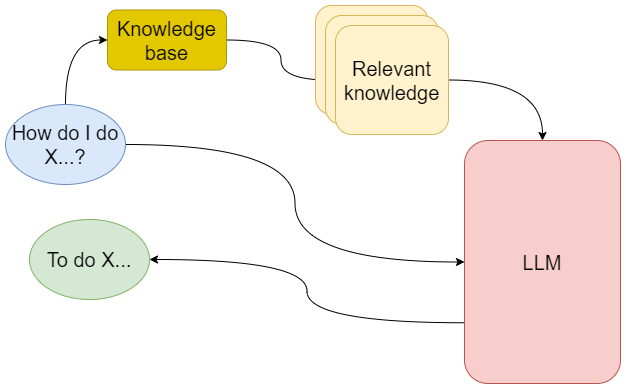
\includegraphics[width=.75\textwidth]{./Figures/RAG.png}
	\caption{Diagrama de flujo de una consulta en un chatbot con arquitectura RAG.}
	\label{fig:arquitectura_rag}
\end{figure}
\vspace{1cm}

  \newpage
  
  \subsection{Fine-Tuning}
  El fine-tuning implica ajustar un modelo de lenguaje preentrenado en un conjunto de datos específico para mejorar su comportamiento en contextos particulares. Este proceso permite que el modelo sea más efectivo en aplicaciones industriales específicas, como medicina, derecho o ingeniería. Sin embargo, una desventaja del fine-tuning es que el modelo resultante puede quedar congelado en un estado particular, limitando su adaptabilidad a nuevos contextos sin un nuevo ciclo de entrenamiento.
  Aunque el fine-tuning proporciona respuestas más precisas en contextos específicos, también puede carecer de la flexibilidad de RAG, que permite incorporar datos contextuales en tiempo real.
   
  \newpage
\subsection{Ventajas y desventajas de los modelos RAG y Fine-Tuning}
  
  Esta subsección presenta una comparación entre ambos modelos, destacando sus ventajas y desventajas.
  \begin{table}[ht]
    \centering
    \begin{tabular}{|c|p{0.35\linewidth}|p{0.35\linewidth}|}
        \hline
        \textbf{Modelo} & \textbf{Ventaja} & \textbf{Desventaja} \\
        \hline
        RAG & 
        \begin{raggedright}
        \begin{itemize}
            \item Permite incorporar información contextual actualizada en tiempo real.
            \item Reduce la probabilidad de alucinaciones al usar datos relevantes.
            \item Mejora la precisión y relevancia de las respuestas del chatbot.
        \end{itemize} 
        \end{raggedright} & 
        \begin{raggedright}
        \begin{itemize}
            \item Requiere una infraestructura adecuada para la recuperación de información.
            \item Dependencia de la calidad y disponibilidad de la base de datos.
            \item Puede ser más complejo de implementar y mantener.
        \end{itemize} 
        \end{raggedright} \\
        \hline
        Fine-Tuning & 
        \begin{raggedright}
        \begin{itemize}
            \item Mejora la calidad de las respuestas al adaptar el modelo a un dominio específico.
            \item Proporciona un rendimiento más consistente en contextos bien definidos.
            \item Permite la optimización de la latencia al trabajar con un modelo entrenado.
        \end{itemize} 
        \end{raggedright} & 
        \begin{raggedright}
        \begin{itemize}
            \item El modelo se congela en el tiempo y no se adapta a cambios contextuales.
            \item Requiere un conjunto de datos específico para el entrenamiento, lo que puede ser costoso.
            \item Menor flexibilidad para abordar consultas inesperadas o no entrenadas.
        \end{itemize} 
        \end{raggedright} \\
        \hline
    \end{tabular}
    \caption{Ventajas y desventajas de los modelos RAG y Fine-Tuning}
    \label{tab:rag_vs_finetuning}
\end{table}



% \chapter{Introducción específica} % Main chapter title

% \label{Chapter2}

% %----------------------------------------------------------------------------------------
% %	SECTION 1
% %----------------------------------------------------------------------------------------
% Todos los capítulos deben comenzar con un breve párrafo introductorio que indique cuál es el contenido que se encontrará al leerlo.  La redacción sobre el contenido de la memoria debe hacerse en presente y todo lo referido al proyecto en pasado, siempre de modo impersonal.

% \section{Estilo y convenciones}
% \label{sec:ejemplo}

% \subsection{Uso de mayúscula inicial para los título de secciones}

% Si en el texto se hace alusión a diferentes partes del trabajo referirse a ellas como capítulo, sección o subsección según corresponda. Por ejemplo: ``En el capítulo \ref{Chapter1} se explica tal cosa'', o ``En la sección \ref{sec:ejemplo} se presenta lo que sea'', o ``En la subsección \ref{subsec:ejemplo} se discute otra cosa''.

% Cuando se quiere poner una lista tabulada, se hace así:

% \begin{itemize}
% 	\item Este es el primer elemento de la lista.
% 	\item Este es el segundo elemento de la lista.
% \end{itemize}

% Notar el uso de las mayúsculas y el punto al final de cada elemento.

% Si se desea poner una lista numerada el formato es este:

% \begin{enumerate}
% 	\item Este es el primer elemento de la lista.
% 	\item Este es el segundo elemento de la lista.
% \end{enumerate}

% Notar el uso de las mayúsculas y el punto al final de cada elemento.

% \subsection{Este es el título de una subsección}
% \label{subsec:ejemplo}

% Se recomienda no utilizar \textbf{texto en negritas} en ningún párrafo, ni tampoco texto \underline{subrayado}. En cambio sí se debe utilizar \textit{texto en itálicas} para palabras en un idioma extranjero, al menos la primera vez que aparecen en el texto. En el caso de palabras que estamos inventando se deben utilizar ``comillas'', así como también para citas textuales. Por ejemplo, un \textit{digital filter} es una especie de ``selector'' que permite separar ciertos componentes armónicos en particular.

% La escritura debe ser impersonal. Por ejemplo, no utilizar ``el diseño del firmware lo hice de acuerdo con tal principio'', sino ``el firmware fue diseñado utilizando tal principio''. 

% El trabajo es algo que al momento de escribir la memoria se supone que ya está concluido, entonces todo lo que se refiera a hacer el trabajo se narra en tiempo pasado, porque es algo que ya ocurrió. Por ejemplo, "se diseñó el firmware empleando la técnica de test driven development".

% En cambio, la memoria es algo que está vivo cada vez que el lector la lee. Por eso transcurre siempre en tiempo presente, como por ejemplo:

% ``En el presente capítulo se da una visión global sobre las distintas pruebas realizadas y los resultados obtenidos. Se explica el modo en que fueron llevados a cabo los test unitarios y las pruebas del sistema''.

% Se recomienda no utilizar una sección de glosario sino colocar la descripción de las abreviaturas como parte del mismo cuerpo del texto. Por ejemplo, RTOS (\textit{Real Time Operating System}, Sistema Operativo de Tiempo Real) o en caso de considerarlo apropiado mediante notas a pie de página.

% Si se desea indicar alguna página web utilizar el siguiente formato de referencias bibliográficas, dónde las referencias se detallan en la sección de bibliografía de la memoria, utilizado el formato establecido por IEEE en \citep{IEEE:citation}. Por ejemplo, ``el presente trabajo se basa en la plataforma EDU-CIAA-NXP \citep{CIAA}, la cual...''.

% \subsection{Figuras} 

% Al insertar figuras en la memoria se deben considerar determinadas pautas. Para empezar, usar siempre tipografía claramente legible. Luego, tener claro que \textbf{es incorrecto} escribir por ejemplo esto: ``El diseño elegido es un cuadrado, como se ve en la siguiente figura:''

% \begin{figure}[h]
% \centering
% \includegraphics[scale=.45]{./Figures/cuadradoAzul.png}
% \end{figure}

% La forma correcta de utilizar una figura es con referencias cruzadas, por ejemplo: ``Se eligió utilizar un cuadrado azul para el logo, como puede observarse en la figura \ref{fig:cuadradoAzul}''.

% \begin{figure}[ht]
% 	\centering
% 	\includegraphics[scale=.45]{./Figures/cuadradoAzul.png}
% 	\caption{Ilustración del cuadrado azul que se eligió para el diseño del logo.}
% 	\label{fig:cuadradoAzul}
% \end{figure}

% El texto de las figuras debe estar siempre en español, excepto que se decida reproducir una figura original tomada de alguna referencia. En ese caso la referencia de la cual se tomó la figura debe ser indicada en el epígrafe de la figura e incluida como una nota al pie, como se ilustra en la figura \ref{fig:palabraIngles}.

% \begin{figure}[htpb]
% 	\centering
% 	\includegraphics[scale=.3]{./Figures/word.jpeg}
% 	\caption{Imagen tomada de la página oficial del procesador\protect\footnotemark.}
% 	\label{fig:palabraIngles}
% \end{figure}

% \footnotetext{Imagen tomada de \url{https://goo.gl/images/i7C70w}}

% La figura y el epígrafe deben conformar una unidad cuyo significado principal pueda ser comprendido por el lector sin necesidad de leer el cuerpo central de la memoria. Para eso es necesario que el epígrafe sea todo lo detallado que corresponda y si en la figura se utilizan abreviaturas entonces aclarar su significado en el epígrafe o en la misma figura.



% \begin{figure}[ht]
% 	\centering
% 	\includegraphics[scale=.37]{./Figures/questionMark.png}
% 	\caption{¿Por qué de pronto aparece esta figura?}
% 	\label{fig:questionMark}
% \end{figure}

% Nunca colocar una figura en el documento antes de hacer la primera referencia a ella, como se ilustra con la figura \ref{fig:questionMark}, porque sino el lector no comprenderá por qué de pronto aparece la figura en el documento, lo que distraerá su atención.

% Otra posibilidad es utilizar el entorno \textit{subfigure} para incluir más de una figura, como se puede ver en la figura \ref{fig:three graphs}. Notar que se pueden referenciar también las figuras internas individualmente de esta manera: \ref{fig:1de3}, \ref{fig:2de3} y \ref{fig:3de3}.
 
% \begin{figure}[!htpb]
%      \centering
%      \begin{subfigure}[b]{0.3\textwidth}
%          \centering
%          \includegraphics[width=.65\textwidth]{./Figures/questionMark}
%          \caption{Un caption.}
%          \label{fig:1de3}
%      \end{subfigure}
%      \hfill
%      \begin{subfigure}[b]{0.3\textwidth}
%          \centering
%          \includegraphics[width=.65\textwidth]{./Figures/questionMark}
%          \caption{Otro.}
%          \label{fig:2de3}
%      \end{subfigure}
%      \hfill
%      \begin{subfigure}[b]{0.3\textwidth}
%          \centering
%          \includegraphics[width=.65\textwidth]{./Figures/questionMark}
%          \caption{Y otro más.}
%          \label{fig:3de3}
%      \end{subfigure}
%         \caption{Tres gráficos simples}
%         \label{fig:three graphs}
% \end{figure}

% El código para generar las imágenes se encuentra disponible para su reutilización en el archivo \file{Chapter2.tex}.

% \subsection{Tablas}

% Para las tablas utilizar el mismo formato que para las figuras, sólo que el epígrafe se debe colocar arriba de la tabla, como se ilustra en la tabla \ref{tab:peces}. Observar que sólo algunas filas van con líneas visibles y notar el uso de las negritas para los encabezados.  La referencia se logra utilizando el comando \verb|\ref{<label>}| donde label debe estar definida dentro del entorno de la tabla.

% \begin{verbatim}
% \begin{table}[h]
% 	\centering
% 	\caption[caption corto]{caption largo más descriptivo}
% 	\begin{tabular}{l c c}    
% 		\toprule
% 		\textbf{Especie}     & \textbf{Tamaño} & \textbf{Valor}\\
% 		\midrule
% 		Amphiprion Ocellaris & 10 cm           & \$ 6.000 \\		
% 		Hepatus Blue Tang    & 15 cm           & \$ 7.000 \\
% 		Zebrasoma Xanthurus  & 12 cm           & \$ 6.800 \\
% 		\bottomrule
% 		\hline
% 	\end{tabular}
% 	\label{tab:peces}
% \end{table}
% \end{verbatim}


% \begin{table}[h]
% 	\centering
% 	\caption[caption corto]{caption largo más descriptivo}
% 	\begin{tabular}{l c c}    
% 		\toprule
% 		\textbf{Especie} 	 & \textbf{Tamaño} 		& \textbf{Valor}  \\
% 		\midrule
% 		Amphiprion Ocellaris & 10 cm 				& \$ 6.000 \\		
% 		Hepatus Blue Tang	 & 15 cm				& \$ 7.000 \\
% 		Zebrasoma Xanthurus	 & 12 cm				& \$ 6.800 \\
% 		\bottomrule
% 		\hline
% 	\end{tabular}
% 	\label{tab:peces}
% \end{table}

% En cada capítulo se debe reiniciar el número de conteo de las figuras y las tablas, por ejemplo, figura 2.1 o tabla 2.1, pero no se debe reiniciar el conteo en cada sección. Por suerte la plantilla se encarga de esto por nosotros.

% \subsection{Ecuaciones}
% \label{sec:Ecuaciones}

% Al insertar ecuaciones en la memoria dentro de un entorno \textit{equation}, éstas se numeran en forma automática  y se pueden referir al igual que como se hace con las figuras y tablas, por ejemplo ver la ecuación \ref{eq:metric}.

% \begin{equation}
% 	\label{eq:metric}
% 	ds^2 = c^2 dt^2 \left( \frac{d\sigma^2}{1-k\sigma^2} + \sigma^2\left[ d\theta^2 + \sin^2\theta d\phi^2 \right] \right)
% \end{equation}
                                                        
% Es importante tener presente que si bien las ecuaciones pueden ser referidas por su número, también es correcto utilizar los dos puntos, como por ejemplo ``la expresión matemática que describe este comportamiento es la siguiente:''

% \begin{equation}
% 	\label{eq:schrodinger}
% 	\frac{\hbar^2}{2m}\nabla^2\Psi + V(\mathbf{r})\Psi = -i\hbar \frac{\partial\Psi}{\partial t}
% \end{equation}

% Para generar la ecuación \ref{eq:metric} se utilizó el siguiente código:

% \begin{verbatim}
% \begin{equation}
% 	\label{eq:metric}
% 	ds^2 = c^2 dt^2 \left( \frac{d\sigma^2}{1-k\sigma^2} + 
% 	\sigma^2\left[ d\theta^2 + 
% 	\sin^2\theta d\phi^2 \right] \right)
% \end{equation}
% \end{verbatim}

% Y para la ecuación \ref{eq:schrodinger}:

% \begin{verbatim}
% \begin{equation}
% 	\label{eq:schrodinger}
% 	\frac{\hbar^2}{2m}\nabla^2\Psi + V(\mathbf{r})\Psi = 
% 	-i\hbar \frac{\partial\Psi}{\partial t}
% \end{equation}

% \end{verbatim}